% standardmäßig im 4:3 Format
% verwende \documentclass[169]{sikslides} für 16:9
\documentclass{sikslides}

\usepackage{bm}
\usepackage{tabu}
\tabulinesep=1.2mm
\usepackage{subcaption}

\newcommand*{\vcenterimage}[2]{\vcenter{\hbox{\includegraphics[height=#1]{#2}}}}
\newcommand*{\vcenterarrow}{\vcenter{\hbox{$\bm{\Longrightarrow}$}}}

\title[Security Considerations for CPS]{Security Considerations for Cyber-Physical Systems}
\subtitle{Seminar \\Cyber-Physical Systems} % Bachelor
%\subtitle{Seminar \\Safety-Critical Systems} % Master
%\subtitle{Seminar Grundlagen\\ moderner Prozessorarchitekturen} % Bachelor
%\subtitle{Seminar Prozessorarchitekturen:\\Aktuelle Forschungstheme} % Master
\author{Maximilian Ammann}
\date[01.02.2019]{01. Februar 2019}
\setbeamercovered{transparent}
\setbeamertemplate{section in toc}[sections numbered]
\setbeamertemplate{subsection in toc}[subsections numbered]
\begin{document}

    \titleframe

    \begin{frame}
        \frametitle{Unterschied von Cybersicherheit und Sicherheit in CPS}
        Anfang Januar: Cybervorfall Doxing ist nicht CPS Sicherheit!
    \end{frame}

    % erneutes Bauen notwendig, um Gliederung zu aktualisieren
    \begin{frame}
        \frametitle{Gliederung}
        %        \tableofcontents[hideallsubsections,pausesections]
        %        \tableofcontents[pausesections]
        \tableofcontents
    \end{frame}

    %    \sectionframe{Eigenschaften von CPS und Angriffsszenarios}
    \section{Eigenschaften von CPS und Angriffsszenarios}

    \begin{frame}[label=abstrakt]
        \frametitle{Abstraktion eines Cyber-physical Systems}
        \begin{figure}
            \centering
            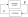
\includegraphics[width=5cm]{../figure/abstrakt}
            \label{fig:abstrakt}
        \end{figure}
    \end{frame}

    \begin{frame}
        \frametitle{Von CIA-Dreieck zu CIAANV-Hexagon?!}
        \centering
        $\vcenterimage{2.5cm}{../figure/cia}\vcenterarrow\vcenterimage{3.5cm}{../figure/triad}$

        \vspace{40px}
        $\rightarrow$ Komplexere Situation bei CPS
    \end{frame}

    \begin{frame}
        <1>[label=eigenschaften]
        \frametitle{Eigenschaften}

        \begin{tabu}
            to \linewidth { | X[1.6,l] | X[5,l] | }
            \hline
            Eigenschaft: $e$&Ein System hat Eigenschaft $e$ genau dann, wenn~\ldots \\
            \hline
            \only<1>{\bf}
            Availability&
            \only<1>{\bf}
            \ldots Ressourcen für autorisierte Teilnehmer angemessen verfügbar ist.\pause \\
            \hline
            \only<2-4>{\bf}
            Confidentiality&
            \only<2-4>{\bf}
            \ldots nur autorisierte Teilnehmer auf Ressourcen zugreifen können.\pause \\
            \hline
            \only<3-4>{\bf}
            Integrity&
            \only<3-4>{\bf}
            \ldots Ressourcen nur von autorisierten Teilnehmern verändert werden können.\pause \\
            \hline
            \only<4>{\bf}
            Authenticity&
            \only<4>{\bf}
            \ldots sich beide Kommunikationspartner einig über die Identität des Gegenübers sind.\pause \\
            \hline
            \only<5>{\bf}
            Veracity und Plausibility &
            \only<5>{\bf}
            \ldots Aussagen des Systems der Wahrhaftigkeit der Wirklichkeit entsprechen. \\
            \hline
            %Non-repudiation &
            %\ldots jedes Ereignis, welches das System beeinflusst, nachvollzogen werden kann. \\
            %\hline
        \end{tabu}
    \end{frame}

    \subsection{Denial-of-Service Angriff}
    \begin{frame}
        <5>
        \frametitle{Szenario: Denial-of-Service Angriff}
        \begin{figure}
            \centering
            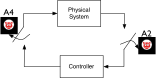
\includegraphics[width=4cm]{figure/dos}
            %            \caption{Abstraktion eines DoS Angriffs}
        \end{figure}
        \begin{itemize}
            \item Ziel: Mit großer Flut an Informationen die \textbf{Availability} des CPS stören
            \item Beispiele:
            \begin{itemize}
                \item CAN Busse in Autos: Fehlfunktion der Warnlichter, Diebstahlsicherung
                \item Echtzeitkritische Stromnetze: Störung des Normalbetrieb
            \end{itemize}
            \item Bei mehreren Angreifern: Distributed-DoS
            \item Kabellose Kommunikation meist anfälliger wegen geringer Bandbreite
        \end{itemize}
    \end{frame}

    \subsection{Man-in-the-Middle Angriff}
    % Continue to Confidentiality, Integrity, Authenticity
    \againframe<2>{eigenschaften}
    \againframe<3>{eigenschaften}
    \againframe<4>{eigenschaften}

    \begin{frame}
        <4>[allowframebreaks]
        \frametitle{Szenario: Man-in-the-Middle Angriff}
        \begin{figure}
            \centering
            \includegraphics[width=4cm]{figure/mitm}
            %            \caption{Abstraktion eines MITM Angriffs}
        \end{figure}
        \begin{itemize}
            \item Passiv: Nur lauschen
            \begin{itemize}
                \item Verletzung der \textbf{Confidentiality} des CPS
            \end{itemize}
            \item Aktiv: Verändern der Daten
            \begin{itemize}
                \item Bei fehlender \textbf{Authenticity}: Keine Verifikation der Identität möglich
                \item Bei fehlender \textbf{Integrity}: Keine überprüfung auf Veränderung der Daten (Prüfsummen!)
            \end{itemize}
        \end{itemize}
        \framebreak
        \begin{itemize}
            \item Beispiele:
            \begin{itemize}
                \item ARP-Poisoning in IEE 802.11 und Local Area Networks
                \item Offline Replay Angriffe bei Autos
            \end{itemize}
        \end{itemize}
    \end{frame}

    \subsection{Angriff auf das physische System}
    % Continue to Veracity
    \againframe<5>{eigenschaften}
    \begin{frame}
        <6>
        \frametitle{Szenario: Angriff auf das physische System}
        \begin{figure}
            \centering
            \includegraphics[width=4cm]{figure/physical}
            %            \caption{Abstraktion eines physischen Angriffs}
        \end{figure}
        \begin{itemize}
            \item Ziel: Verändern der Daten bevor diese an das Cybersystem geschickt werden
            \item \textbf{Authenticity} hilft nicht Veracity sicherzustellen
            \item Beispiele:
            \begin{itemize}
                \item Manipulation von physischen Prozessen führt zu Wechselwirkungen
                \item Manipulation von Sensoren
            \end{itemize}
        \end{itemize}
    \end{frame}

    % Continue to Non-repudiation
    % \againframe<6>{eigenschaften}

    \sectionframe{Gegenmaßnahmen}
    \subsection{Proaktive Maßnahmen: Verhindern von Angriffen}
    \begin{frame}
        \frametitle{Proaktive Maßnahmen: Verhindern von Angriffen}
        Proaktive Maßnahmen: Verhindern von Angriffen
    \end{frame}
    \subsection{Reaktive Maßnahmen: Detektion und Wiederherstellung}
    \begin{frame}
        \frametitle{Reaktive Maßnahmen: Detektion und Wiederherstellung}
        Reaktive Maßnahmen: Detektion und Wiederherstellung
    \end{frame}

    \sectionframe{Zusammenfassung}
\end{document}

